\documentclass[tikz,border=5pt]{standalone}
\usepackage[T1]{fontenc}
\usepackage{lmodern}
\usetikzlibrary{arrows.meta,shapes.geometric}

\begin{document}
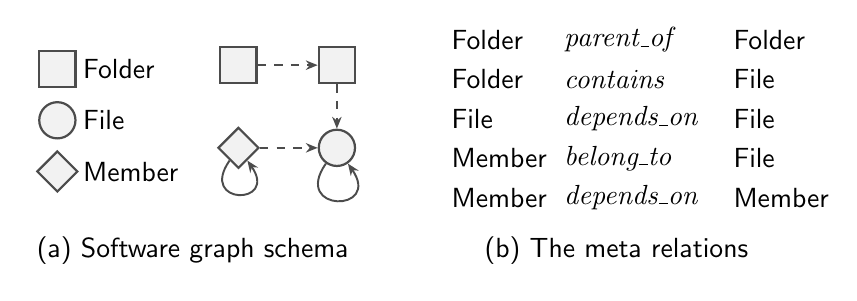
\begin{tikzpicture}[
  x=1cm,y=1cm,
  font=\sffamily\normalsize, %\sffamily
  folder/.style={rectangle,draw=black!70,fill=gray!10,
    line width=.8pt,minimum size=4.6mm,inner sep=0pt},
  file/.style={circle,draw=black!70,fill=gray!10,
    line width=.8pt,minimum size=4.6mm,inner sep=0pt},
  member/.style={diamond,aspect=1,draw=black!70,fill=gray!10,
    line width=.8pt,minimum size=5.2mm,inner sep=0pt},
  relation/.style={-{Stealth[length=1.5mm,width=1.2mm]},
    draw=black!70,line width=.7pt,dashed},
  dependency/.style={-{Stealth[length=1.5mm,width=1.2mm]},
    draw=black!70,line width=.7pt},
  label/.style={anchor=west,inner sep=0pt}
]

% Node-type legend.
\node[folder] at (0,2.00) {};
\node[label] at (.32,2.00) {Folder};
\node[file] at (0,1.35) {};
\node[label] at (.32,1.35) {File};
\node[member] at (0,.70) {};
\node[label] at (.32,.70) {Member};

% (a) Software graph schema.
\node[folder] (parent) at (2.30,2.05) {};
\node[folder] (child) at (3.55,2.05) {};
\node[file] (sourcefile) at (3.55,1.00) {};
\node[member] (sourceMember) at (2.30,1.00) {};

\draw[relation] (parent) -- (child);
\draw[relation] (child) -- (sourcefile);
\draw[relation] (sourceMember) -- (sourcefile);

% Rounded dependency loops.
\draw[dependency]
  (sourcefile) edge[loop below,out=235,in=305,
    looseness=7,min distance=7mm] (sourcefile);

\draw[dependency]
  (sourceMember) edge[loop below,out=235,in=305,
    looseness=7,min distance=7mm] (sourceMember);

\node at (1.72,-.30) {\normalsize (a) Software graph schema};

% (b) Typed relations: source, relation, target.
\foreach \yy/\src/\rel/\dst in {
  2.37/Folder/parent\_of/Folder,
  1.87/Folder/contains/File,
  1.37/File/depends\_on/File,
  .87/Member/belong\_to/File,
  .37/Member/depends\_on/Member
}{
  \node[label] at (5.00,\yy) {\src};
  \node[label,font=\normalsize\itshape] at (6.43,\yy) {\rel}; %\sffamily\
  \node[label] at (8.58,\yy) {\dst};
}

\node at (7.10,-.30) {\normalsize (b) The meta relations};

\end{tikzpicture}
\end{document}